\documentclass{../template/texnote}

\title{\textbf{\capitalisewords{The Galaxy Revelation and a Growing Universe}}}%[author={Linn Abraham}]

\begin{document}
    \maketitle \currentdoc{note}
    %<*note>


\section{What are Nebulae? }

Imagine looking out into the night sky with just your eyes and seeing hundreds upon hundreds of small and big stars spread out over the night sky. By consistently observing some of these over several weeks or months we can identify the planets which have a different motion in the sky. On closer observation we can find several hazy patches of light in the sky. Andromeda (M31) is one such example of a fuzzy and extended object, the Large and Small Magellanic clouds being the other.  All such objects were termed 'nebulae' by the early astronomers. What are these strange fuzzy objects seen in the sky? What makes them different? 

On days that are clear or with a long exposure photograph something else becomes visible. A band of light in the sky which the ancient greeks called the "Milky way". The term "galaxy" is greek for milky circle. When our telescopes improved we could see that rather than being a diffuse cloud the milky way consisted of a vast collection of stars flattened into a disk like structure seen edge-on. 

Returning to our discussion of nebulae, in modern astronomy the term nebulae is now reserved for vast clouds of gas and dust in space. Thus all of the nebulae that were visible to early astronomers were not in fact nebulae. Although there are a few nebulae that are visible in the night sky like the Orion nebulae.  Of the other type of nebulae that were visible to early astronomers, the most common were the spiral shaped nebulae. 

\begin{figure}
     \centering
     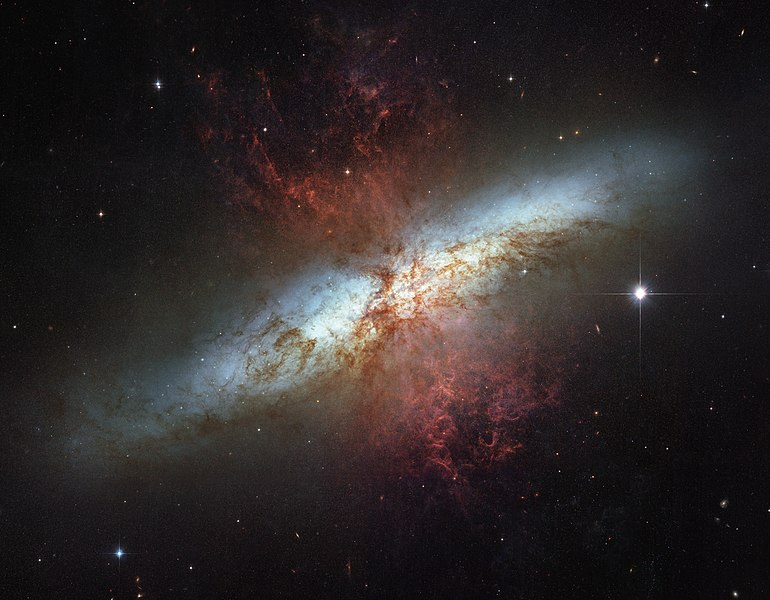
\includegraphics[width=\textwidth]{Linn/M82_HST_ACS_2006-14-a-large_web.jpg}
     \label{fig:cigar}
     \caption{ Messier 82 (also known as NGC 3034, Cigar Galaxy or M82) is a starburst galaxy approximately 12 million light-years away in the constellation Ursa Major. The figure is a mosaic image taken by the Hubble Space Telescope of Messier 82, combining exposures taken with four colored filters that capture starlight from visible and infrared wavelengths as well as the light from the glowing hydrogen filaments. }
 \end{figure}
 
\begin{figure}
     \centering
     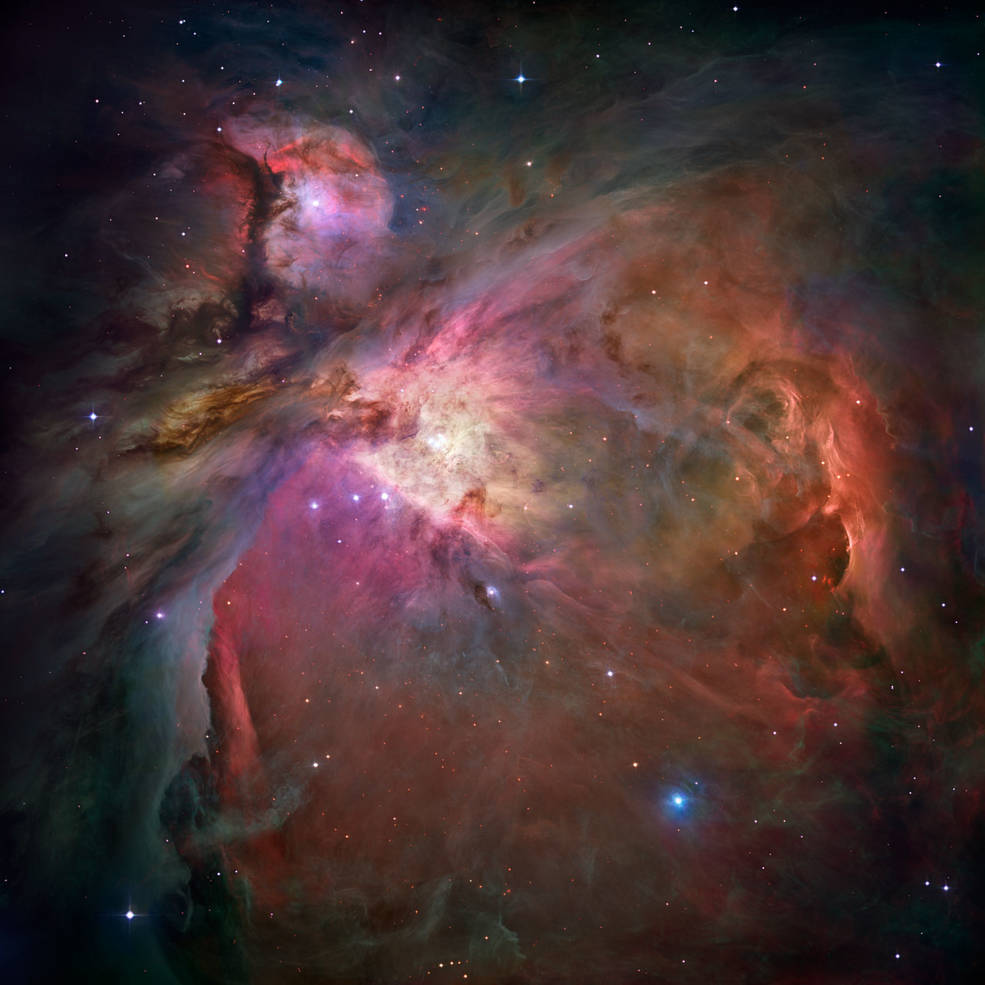
\includegraphics[width=\textwidth]{Linn/orion-nebula-xlarge_web.jpg}
     \label{fig:orion}
     \caption{The entire Orion Nebula in a composite image of visible light and infrared; taken by Hubble Space Telescope in 2006}
 \end{figure}
 
 

\section{Galaxies Within Galaxies: The Island Universe Hypothesis}

There is a story about how our understanding of the size of the visible universe changed sharply after the 1920's. Until then the Milky-way galaxy was thought to be the entire universe.  It all started with the well known philosopher Immanuel Kant who speculated  that some of the faint cloudy patches observed in the night sky might be separate "island universes" distinct from our own. This hypothesis turned from just a hypothesis into a fully blown debate among astronomers as more data and observations poured in. 

The Great Debate in astronomy also called the Shapley-Curtis debate of 1920 was precisely on this topic. Harlow Shapley is the astronomer who is credited with discovering the true shape and size of our own Galaxy. Shapley believed that these nebulae were relatively small and lay within the bounds of our own universe, while Curtis held that they were in fact independent galaxies, very large but distant. 

 \begin{figure}
     \centering
     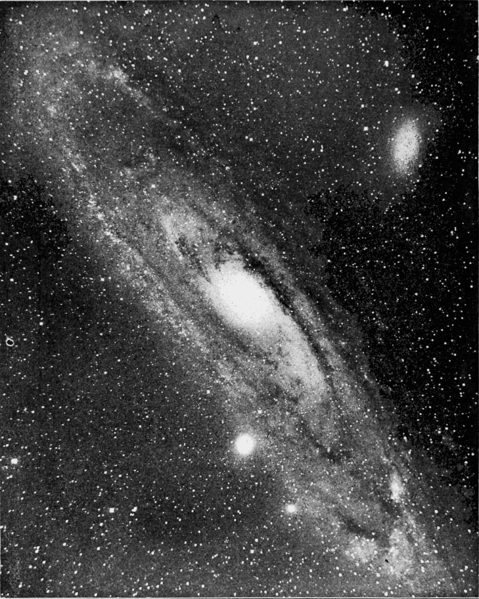
\includegraphics[width=0.65\textwidth]{Linn/479px-PSM_V60_D298_Great_nebula_in_andromeda.png}
     \label{fig:spiral}
     \caption{The "Great Spiral Nebula" in the constellation Andromeda (1902 photograph). The Debate was over whether this was a cloud of gas and dust or a distant galaxy.}
 \end{figure}
 
 
 
\section{Edwin Hubble Settles the Dust}

Henrietta Levitt's discovery of the period-lumniosity relationship for Cepheid variables in the Small Magellanic Clouds was critical to solving the debate.  In the later part of the year 1920, Edwin Hubble used the 100-inch Hooker Telescope at Mount Wilson Observatory, which was the largest operational telescope at the time to observe Cepheids in the Andromeda nebulae. He  used them as distance indicators and measured the distance to the nebulae using those. He found that the Andromeda nebulae was many times more distant than the majority of stars visible in the night sky. He thus established that Curtis was right and that Immanuel Kant's speculations were justified. We now know that our Milky Way is just one out of the 2 trillion or more galaxies in the observable universe. 

\section{Galaxies that are Moving Away from Us}

Although the redshift of starlight was observed before Hubble, Edwin Hubble systematically observed galaxies and measured their distances using the same technique that he used for establishing the size of the Universe. He then analyzed their redshift and derived the famous Hubble Law which showed that all galaxies are moving away from us at an accelerating pace propotional to the distance towards them. The Andromeda galaxy is an exception to this and scientists now believe that the Andromeda galaxy is on a collision course towards our own galaxy. 

\section{The Mystery Continues.. }

Today we know that the nebulae that early astronomers observed are actually galaxies. Vast cities of stars, gas and dust floating in space just like the one in which we are living. However
even after 100 years since Hubble's discoveries and more detailed observations of galaxies, there is still a lot more to be known about them. The wide variety of shapes that they come in puzzle astronomers to this day. Even though Hubble showed that the millions of galaxy shapes can be reduced to a few categories (The Hubble Classification system), there is still no underlying theory that can explain all the features that are observed in galaxies. 


 \begin{figure}
     \centering
     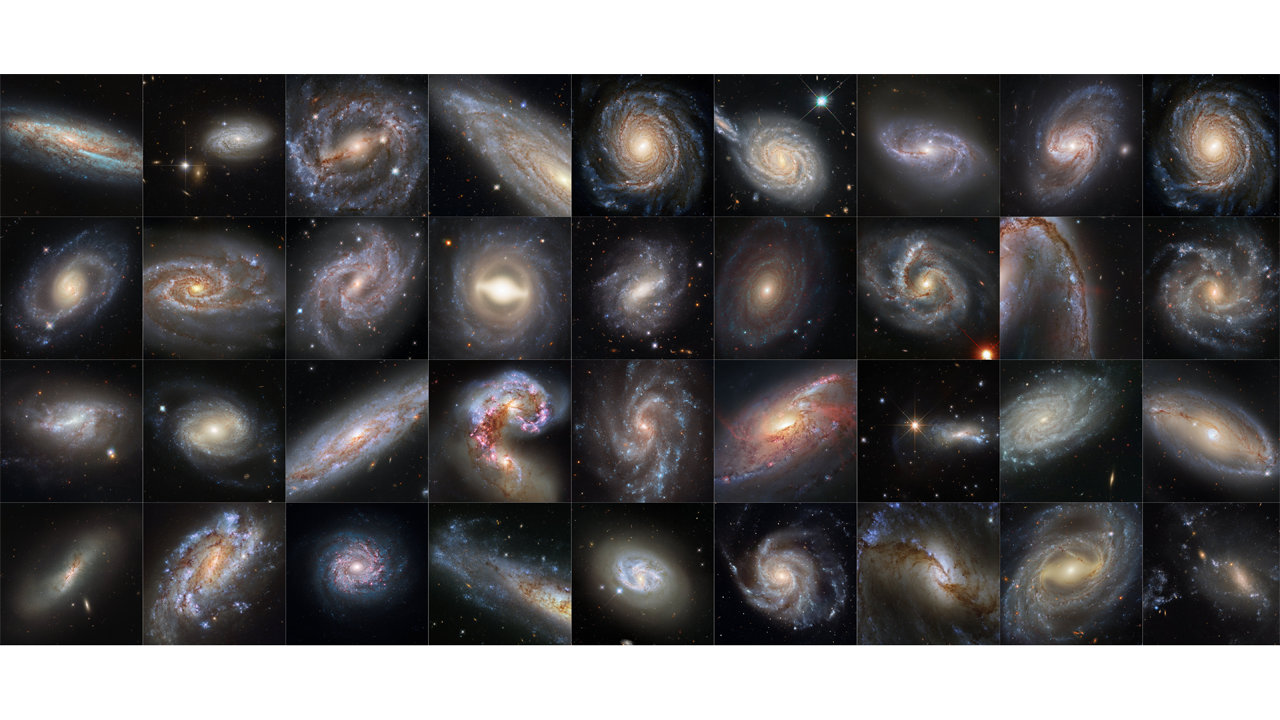
\includegraphics[width=\textwidth]{Linn/STScI-01G2QPZAZGX3NY83EM9GJHT9GT.png}
     \label{fig:mozaic}
     \caption{The Hubble Space Telescope Galaxy collection showing the variety of galaxy shapes. Image Credit: NASA}
 \end{figure}


\begin{figure}
     \centering
     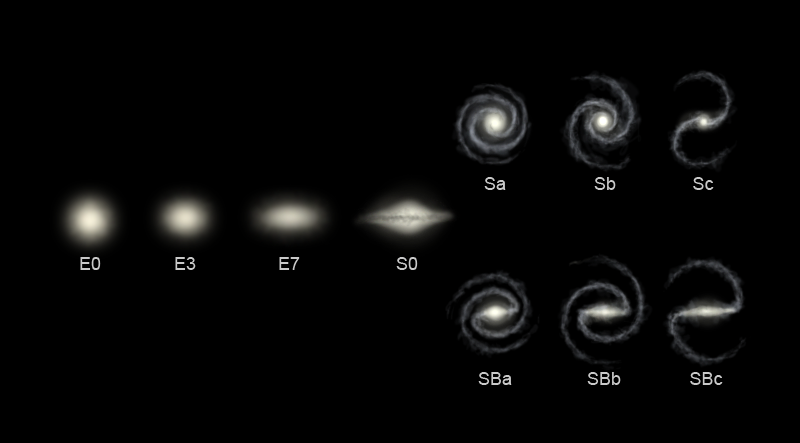
\includegraphics[width=\textwidth]{Linn/Hubble_sequence_photo.png}
     \label{fig:tuning-fork}
     \caption{The Hubble sequence: classification of galaxies. Image Credit: Wikipedia.org}
 \end{figure}

\section{References}
\begin{enumerate}
\item Shu, Frank H. The Physical Universe: An Introduction to Astronomy. 9. print. A Series of Books in Astronomy. Sausalito, Calif: Univ. Sience Books, 1982.

\item Rai, Choudhuri Arnab. Astrophysics for Physicists.

\item Whitrow, G. J. ``Kant and the Extragalactic Nebulae'' 8 (March 1967): 48.



\end{enumerate}

\vspace{0.5cm}
\noindent\fbox{%
	\parbox{\textwidth}{%
		\textbf{About the Author}\vspace{0.2cm} \\
		\textbf{Linn Abraham} is a researcher in Physics, specializing in A.I. applications to astronomy. He iscurrently involved in the development of CNN based Computer Vision tools for classifications of astronomicalsources from PanSTARRS optical images. He has used data from a several large astronomical surveys includingSDSS, CRTS, ZTF and PanSTARRS for his research.
		
	}
}
    %</note>
    \printbibliography
\end{document}
